\documentclass[10pt,a4paper]{scrartcl}
\pagestyle{empty}
\usepackage{a4} % alternativ \usepackage{a4wide}
\usepackage[ngerman]{babel} % Neudeutsche Silbentrennung (mehrsprachiges Dokument)
\usepackage{parskip} % Skip indentation of first row
\usepackage{graphicx} % Graphics support
\usepackage{longtable} % Tables across several pages
\usepackage{booktabs}
\usepackage{hyperref} % Hyperlinks
\usepackage[automark]{scrpage2} %kopf/fusszeile
\usepackage[utf8x]{inputenc} % Unicode-Encoding
 
\linespread{1.3}

\author{Danilo Bargen, Christian Fässler, Jonas Furrer} 
\title{Code-Metriken und Design-Analyse Backend\\ Projekt BierIdee}

\pagestyle{scrheadings}
\ihead{SE2 Projekte} %linke Kopfzeile
\ohead{BierIdee} %rechte Kopfzeile

\begin{document}

\begin{titlepage}
	\maketitle
	\vspace{120mm}
	\thispagestyle{empty} % Don't start page numbers on this page
\end{titlepage}

\tableofcontents
\newpage

\section*{Änderungshistorie}
\begin{tabular}{p{0.1\textwidth}p{0.15\textwidth}p{0.55\textwidth}p{0.1\textwidth}}
\toprule
\textbf{Version} & \textbf{Datum} & \textbf{Änderung} & \textbf{Person} \\  
\midrule
v1.0 & 08.05.2012 & Dokument erstellt & jfurrer \\  
\bottomrule
\end{tabular} 
\newpage

\section{Einführung}

\subsection{Zweck}
In diesem Dokument werden die Code Metriken des Projektes BierIdee betrachtet und analysiert.

\subsection{Gültigkeitsbereich}
Die Gültigkeit des Dokumentes beschränkt sich auf die Dauer des SE2-Projekte Modules FS2012. Das
Dokument muss unter Berücksichtigung des Wachstums der Code-Basis ergänzt und erweitert werden.

\subsection{Tools}
Für die Analyse werden die folgende Tools verwendet:\\
\begin{itemize}
	\item Checkstyle
	\item Metrics Eclipse Plugin
	\item AnalytiX CodePro Tools
	\item Object Aid
\end{itemize}

\newpage

\section{Package Diagramm}
\subsection{Interpackage Dependencies}
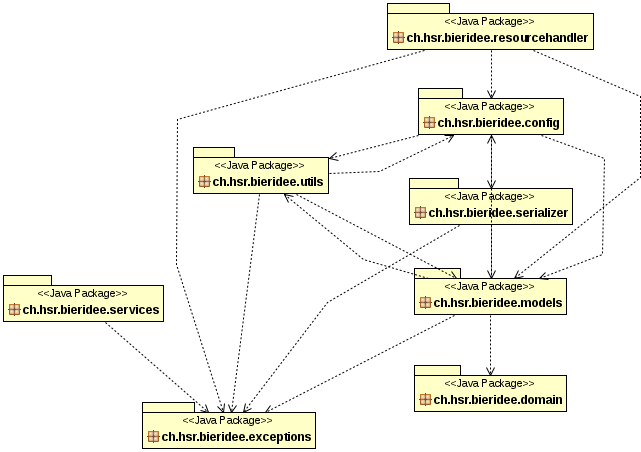
\includegraphics[width=\textwidth]{Package-Diagramm.png}\\
\\
Die Packages zeigt die Stuktur des Backends deutlich auf, die Resource-Handler greifen  
auf die Models zu um Daten zu lesen und zu Persisteren. Die Models greifen dann über Utilities
auf die Daten zu und persistieren die Domainobjekte.\\
Die Konfigurationen aus dem Config Package sowie die Exceptions werden von den meisten anderen
Packages benötigt.

\subsubsection{External Dependencies}
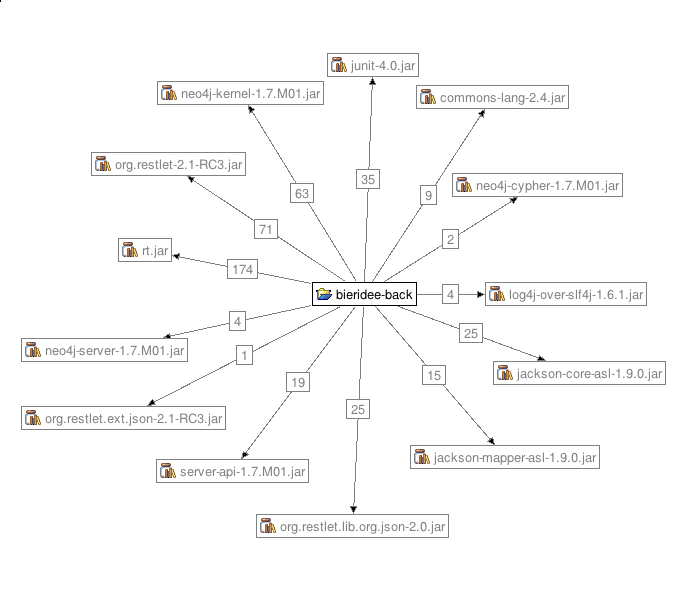
\includegraphics[scale=0.7, width=\textwidth]{dependecies.png}\\
\\
Durch die Verwendung von Restlet enstehen relativ viele externe Abhängigkeiten.

\section{Metriken}
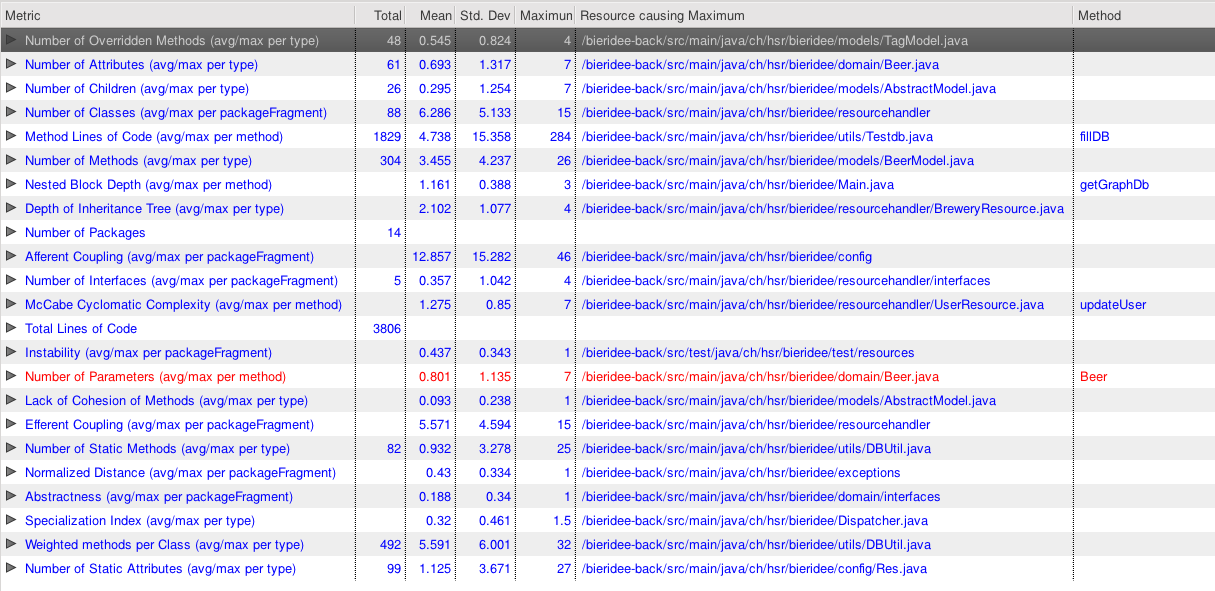
\includegraphics[scale=0.5, angle=90]{metrics.png}



\end{document}
